\documentclass[12pt]{jsarticle}
%
\usepackage{amsmath,amssymb}
\usepackage{bm}
\usepackage[dvipdfmx]{graphicx}
\usepackage{subfigure}
\usepackage{verbatim}
\usepackage{wrapfig}
\usepackage{ascmac}
\usepackage{makeidx}
%
\setlength{\textwidth}{\fullwidth}
\addtolength{\textheight}{\topskip}
%Math
\newcommand{\diff}{\mathrm{d}}  %微分記号
\newcommand{\divergence}{\mathrm{div}\,}  %ダイバージェンス
\newcommand{\grad}{\mathrm{grad}\,}  %グラディエント
\newcommand{\rot}{\mathrm{rot}\,}  %ローテーション
%Title
\title{平成27年度 修士論文  \\ \\ ハイブリッドロケット液体酸素気化に関する研究}
\author{東海大学大学院工学研究科\\航空宇宙学専攻\\学生番号:4bmjm020 三島源生\\ \\ \\指導教員:}
\date{\large{2016/2}}
\begin{document}
\maketitle
%\newpage
\chapter*{概要}
\ 
考え中
\\

%\section*{\large 問題1}
\ 
配布資料より、各パラメータは以下のようになる。
\begin{table}[htb]
 \begin{center}
  \caption{各仮定値及びJR100のパラメータ}
  \begin{tabular}{|l|r|} \hline
   \multicolumn{2}{|c|}{|JR100|} \\ \hline
   推力比:$sigma$ (=$\frac{V_n}{V_j}$,$V_n=0$)[-] & 0 \\ \hline
   低圧タービン断熱効率:$\eta_t$ [-] & 0.88 \\ \hline
   ファン断熱効率:$eta_f[-]$ & 0.852 \\ \hline
   バイパス効率:$eta$[-] & 0.74976 \\ \hline
   圧縮機での定圧比熱:$c_{pc} [j/kg K]$ & 1004 \\ \hline
   タービン及びノズルでの定圧比熱:$c_{pt} [J/kg K]$ & 1155 \\ \hline
   圧縮機入口全温:$T_t[K]$ & 288.2 \\ \hline
   タービン出口全温:$T_{t4}[K]$ & 983.2 \\ \hline
   排気静温:$T_{j}[K]$ & 840 \\ \hline
   圧縮機比熱比:$\kappa_c [-]$ & 1.4 \\ \hline
   $\kappa_c/{\kappa_c -1}$ & 3.5 \\ \hline
  \end{tabular}
 \end{center}
\end{table}
また、最適エネルギー分配率$\lambda_{op}$及び、最適推力比$\tau_{op}$を求める式は、
\begin{equation}
 \lambda_{op}=\frac{\mu(\eta^2-\sigma^2)}{\eta(1+\mu \eta)}
\end{equation}
\begin{equation}
 \tau_{op}=\frac{\sqrt{1-\lambda_{op}} -\sigma +(\sqrt{\mu(\mu\sigma^2+\eta\lambda_{op})}-\mu\sigma)}{1-\sigma}
\end{equation}
である。これより得た最適エネルギー分配率$\lambda_{op}$及び最適推力比$\tau_{op}$の値を以下に示す。
\begin{table}[htb]
 \begin{center}
  \caption{各バイパス比にエネルギーおける最適エネルギー分配率及び最適推力比}
  \begin{tabular}{|r|r|r|} \hline
  バイパス比$\mu$ [-] & 最適エネルギー分配率$\lambda_{op} [-] $ & 最適推力比$\tau_{op}[-]$   \\ \hline
  0  & 0            &  1            \\ \hline
  1  & 0.42849305   &  1.322784941  \\ \hline
  2  & 0.599923185  &  1.580987033  \\ \hline
  6  & 0.818134202  &  2.344900851  \\ \hline
  10 & 0.882319714  &  2.915064322  \\ \hline
  15 & 0.91834335   &  3.499485676  \\ \hline
  20 & 0.937481244  &  3.999399955  \\ \hline
  \end{tabular}
 \end{center}
\end{table}
\\
\begin{figure}[t]
 \begin{center}
  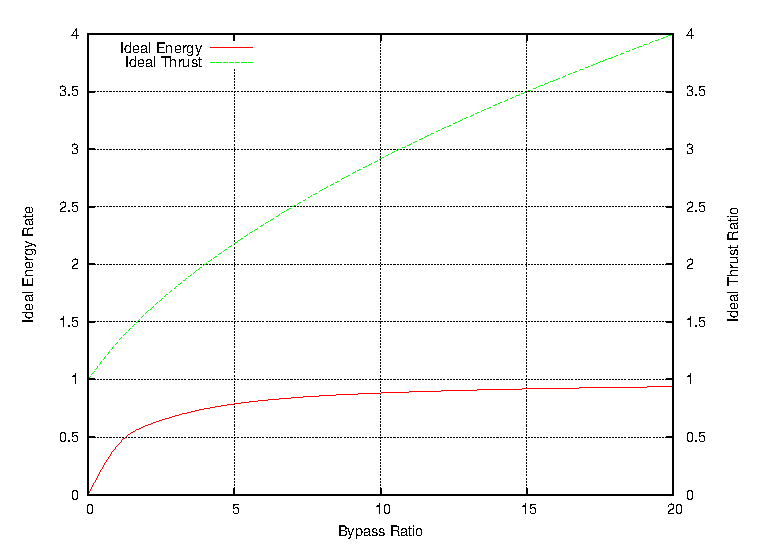
\includegraphics[width=10.0cm]{eps/body1_1.eps}
  \caption{バイパス比との関係}
 \end{center}
\end{figure}

%\begin{equation}
%\alpha M = F
%\end{equation}
%\\
%\begin{figure}[b]
% \begin{center}
%  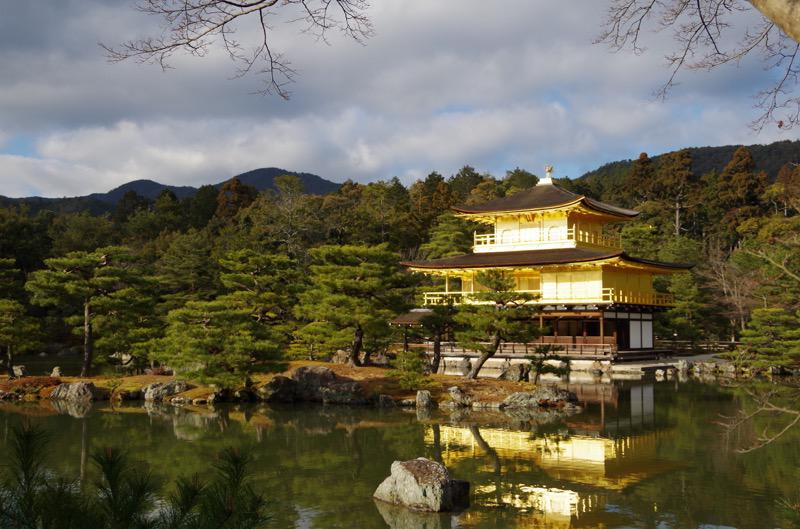
\includegraphics[width=7.0cm]{png/apple.eps}
%  \caption{Title}
%  \label{label}
% \end{center}
%\end{figure}
\\

%\section*{\large 問題2}
\ 
ファン圧力比$\pi_f$を求める式は、
\begin{equation}
 \pi_f = \left\{\frac{c_{pt}(T_{t4}-T_j)\lambda_{op} \eta}{c_{pc}T_{t1}\mu}+1\right\}^{\frac{\kappa_c}{\kappa_c-1}}
\end{equation}
となる。これより得たファン圧力比$\pi_f$の値を以下に示す。
\begin{table}[htb]
 \begin{center}
  \caption{各バイパス比におけるファン圧力比}
  \begin{tabular}{|l|r|} \hline
    バイパス比$\mu [-]$  &  最適 ファン圧力比  $\pi_f [-]$ \\  \hline
                      0  &   -                             \\  \hline
                      1  &   1.804124844                   \\  \hline
                      2  &   1.526961406                   \\  \hline
                      6  &   1.219912007                   \\  \hline
                      10 &   1.138721282                   \\  \hline
                      15 &   1.094885139                   \\  \hline
                      20 &   1.072093843                   \\  \hline
   
  \end{tabular}
 \end{center}
\end{table}

\begin{figure}[t]
 \begin{center}
  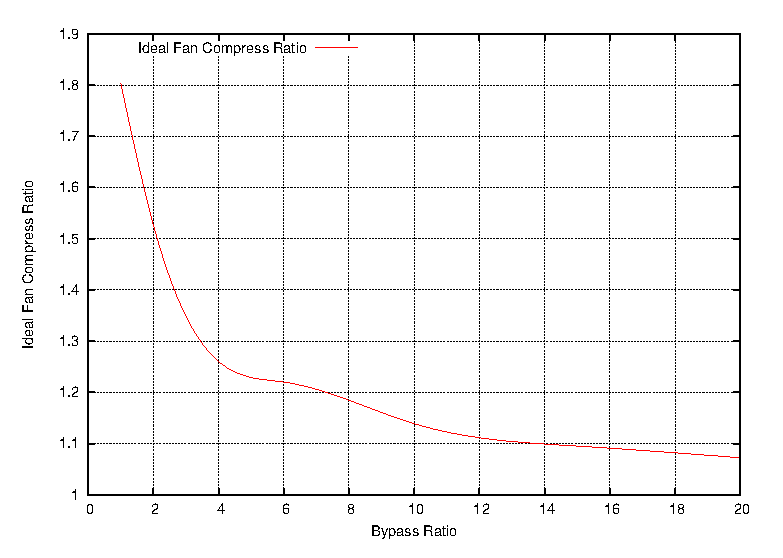
\includegraphics[width=10.0cm]{eps/body2_1.eps}
  \caption{バイパス比との関係}
 \end{center}
\end{figure}

%\section*{\large 問題3}
\ 
バイパス比が$\mu=0$の場合、エネルギー分配率$\lambda$が$0$の時に推力比$\tau$は1となる。エネルギー分配率は、ターボファンエンジンにおいてファンによって発生した低速排気ジェットのエネルギーとコアエンジンを介した燃焼ガスのエネルギーとの割合なので、バイパス比$\mu=0$では、ファンを通した空気の流れ全てがコアエンジンを通り、燃焼ガスとして推力になると考えられる。従って推力比1というのは燃焼ガスによる推力が$100%$損失ないことを意味し、$\tau$は全推力のうちの、燃焼ガスが占める割合を表す。また、推力の全てを燃焼ガスがまかなっている状態は、ターボジェットエンジンと同等の状態であると考えられる。一方で、エネルギー分配率$\tau$が1の場合は、理論的には推力全体をファンによって発生した空気の流れが占めていると考えられる。これは、ガスタービンの燃焼ガスが推力にほぼ影響を与えず、タービンに寄ってくどうしたプロペラによって推力を得るターボプロップエンジンとほぼ同じ状態となる。

\end{document}
